\section{\texorpdfstring{Latinské čtverce}{Latinské čtverce}}
\vspace{5mm}
\large

\begin{definition}
	Latinský obdélník je matice $L \in X^{k \times n}$. Taková, že prvky se neopakuji ani ve sloupcích ani v řádcích.
	Kde $X$ je n-prvková množina. Typický $\{ 1, ..., n \} := [n]$.

	Na řádky lze nahlížet jako na permutace.
\end{definition}

\begin{theorem}[Latinské čtverce]
	Každý Latinský obdélník řádu $k \times n$ lze doplnit na Latinský čtverec řadu $n \times n$.
\end{theorem}
\begin{proof}
	Dokážeme přidaní nových řádků v závislostí na již existujících řádcích.

	V k-tem kroků se podíváme na j-tý sloupec.
	Nechť $M_j$ bude množina kandidátů které můžeme dat na j-tou pozici v novém řádku.
	\[ M_j = [n]\setminus \{ L_{ij}: i = 1, 2, ... , k \} \]

	Teď musíme z množin $M_j$ vzít po 2 různé prvky.
	Jinými slovy, hledáme Systém různých reprezentantů - SRR pro $\{ M_j \}_1^n$.

	Sestavíme graf, kde vrcholy jsou množiny $M_j$ a prvky z $[n]$.
	\[ (l, M_j) \in E \iff l \in M_j \]

	Pak tento bipartitní graf je $(n - k)$-regulární.
	Protože $\forall x$ je v $(n - k)$ množinách $M_j$.

	Dle Hallové věty, v takovém grafu existuje perfektní párovaní, které určuje SRR.
\end{proof}

\begin{consequence}
	Latinských čtverců řádu $n$ je $\bigO(n!)$.
\end{consequence}
\begin{proof}
	BUNO: v prvním řádku je $\{ 1, 2, ..., n \}$.
	Jinak můžeme vhodně přejmenovat prvky.

	V druhém řádku musí být permutace $[n]$ bez pevných bodů.
	Z \emph{problému šatnářky} takových permutaci je
	\[ \frac{n!}{e} \]
	Pak dle věty každý obdélník lze doplnit na čtverec.
\end{proof}

\begin{definition}
	Latinský čtverce jsou kolmé $L \perp L^{\prime}$ právě když
	\[ \forall x,y \in [n]^2 \exists ! (i,j) \in [n]^2: L_{i,j} = x \land L_{i,j}^{\prime} = y \]

	Taky lze definovat ortogonalitu nad různými množiny.
\end{definition}

\begin{notation}
	$NOLČ(n)$ značíme největší počet navzájem ortogonálních Latinských čtverců řádu $n$.
\end{notation}

\begin{theorem}[Horní odhad NOLČ]\label{nolc_lower0}
	\[\forall n \in \N, n > 1: NOLČ(n) \leq n - 1 \]
\end{theorem}
\begin{proof}
	Nechť
	\[L^1, ..., L^t \in \{ 1, ..., n \}^{n \times n}, \forall i \neq j: L^i \perp L^j \]

	BUNO: přejmenujeme prvky v každém LČ tak, aby v prvním řádku bylo $\{ 1, 2, ..., n \}$.
	Takto vyrobíme LČ $L^{1 \prime}, ..., L^{t \prime}$.

	Tvrdíme ale, že ortogonalita je zachovaná.
	Obecně pro libovolná permutace $\pi$ aplikovaná ne jeden z dvojice ortogonálních LČ zachovává ortogonalitu.

	Pak na pozici $(2,1)$ nemůže být 1.
	Pokud tam ale bude nějaké písmeno $a$, tak čtverce nebudou ortogonální, protože všechny dvojice $(i, i)$ máme v prvním řádku.
	Z toho na pozice $(2,1)$ můžou být prvky $\{ 2, ..., n \}$ po 2 různé.
	Takže $NOLČ(n) \leq n - 1 $.
\end{proof}

Kdy máme extremální řešení?

\begin{theorem}[Extremální NOLČ a KPR]
	\[ NOLČ(n) = n - 1 \iff \exists KPR(n) \]
	Z předchozí přednášky platí pro mocniny prvočísla.
\end{theorem}
\begin{proof}
	$KRP \Rightarrow LČ$. Sestavíme nevlastní přímku A, svislé a vodorovné přímky.
	Dal přímky spojující A a průniky svislých a vodorovných přímek budou určovat LČ.
	\[ L^{\alpha}_{i,j} = \beta \iff x_{i,j} \in k_{\alpha, \beta} \]

	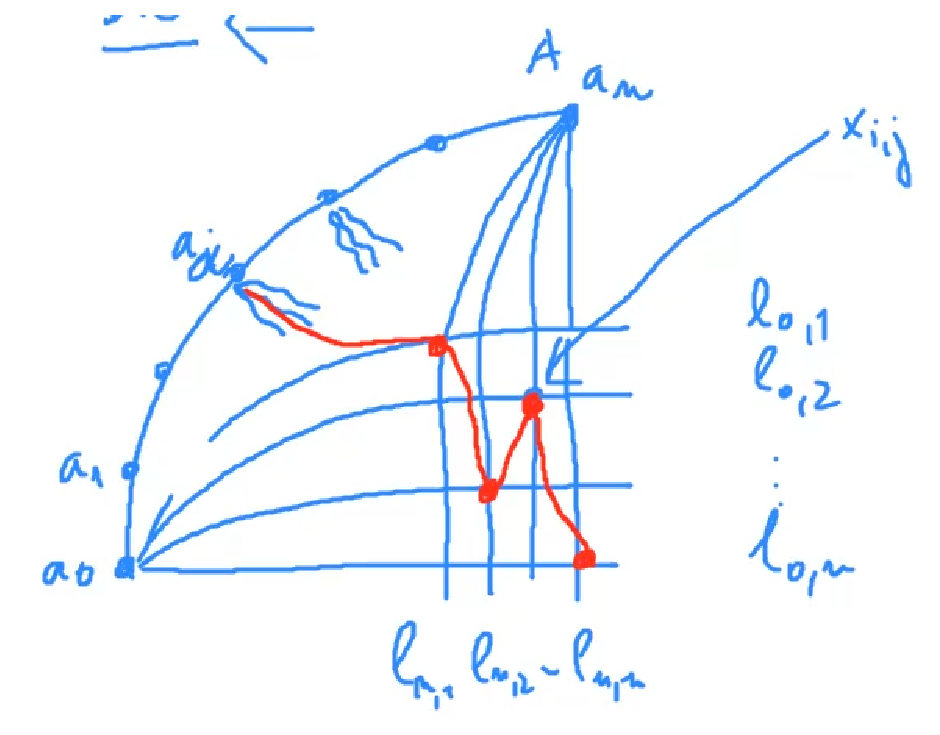
\includegraphics[scale=0.3]{lc_0.eps}

	Pak písmena v LČ odpovídající červené přímce budou:

	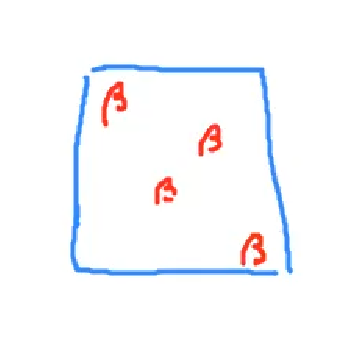
\includegraphics[scale=0.4]{lc_1.eps}

	Z axiomu KPR svislé, vodorovné a přímky procházející body $a_{\alpha}$ se protínají právě v 1 bodě.
	Takže písmena se neopakuji v rádcích a sloupcích.

	Jsou $\perp$ protože
	\[ \forall \beta, \beta^{\prime} \exists ! (i, j): L^{\alpha}_{i, j} = \beta \land L^{\gamma}_{i,j} = \beta^{\prime} \]
	Protože přímky se nemůžou protínat na nevlastní přímce A, takže se protínají uvnitř šachovnice.
	\[ \exists ! x_{i, j} \in l_{\alpha, \beta} \cap l_{\gamma, \beta^{\prime}} \]

	$LČ \Rightarrow KPR$. Nechť máme LČ
	\[ L^{\alpha}, \alpha \in \{ 1, 2, ... ,n - 1 \} \]
	Sestavíme nevlastní, svislé a vodorovné přímky.

	Šikmé přímky vytvoříme dle:
	\[ L^{\alpha}_{i,j} = \beta \iff x_{i,j} \in k_{\alpha, \beta} \]

	Ověříme axiomy:
	\begin{itemize}
		\item $A_1$. Přímky ze stejného svazku šikmých přímek se protínají v nevlastním bodě.
			Vodorovné a svislé se protínají v šachovnici.

			Šikmé vs svislé a Vodorovné vs svislé se protínají protože průniky jsou určené LČ.
			2 Šikmé přímky se protínají právě v 1 bodě protože čtverce jsou $\perp$.
		\item $A_3$. Plyne z toho, že $n \geq 2$.
		\item $A_2$. Spočítáme 2ma způsoby \# 3jic.
			\[ T = |\{ ((x,y), l): x \ne y \in X, l \in L, x,y \in l \}| \]
			Máme $(n^2 + n + 1)$ přímek, na každé z nich je $(n + 1)$ bodů. Pak
			\[ T = (n^2 + n + 1) \binom{n + 1}{2} \]
			Na druhou stranu, máme $(n^2 + n + 1)$ bodů. Každou 2ci prochází nejvýše 1 přímka.
			\[ T \leq 1 \cdot \binom{n^2 + n + 1}{2} \]
			Dohromady
			\[ (n^2 + n + 1) \binom{n + 1}{2} \leq \binom{n^2 + n + 1}{2} \]
			Po roznásobení dostaneme stejná čísla na obou stranách, což může nastat pouze v případě že každou 2cí bodů prochází \emph{právě 1} přímka.
	\end{itemize}
\end{proof}

\begin{definition}
	Ortogonální tabulka řádu $n$, hloubky $d$ je matice
	\[ M \in \{ 1, ..., n \}^{d \times n^2} \]
	$d$ řádků, $n$ sloupců.
	Každé 2 řádky jsou ortogonální. Formálně:
	\[ \forall i \neq j, \forall x,y \in [n], \exists !k \in \{ 1, ..., n^2 \}: M_{i, k} = x \land M_{j, k} = y \]
\end{definition}

\begin{note}
	Jelikož počet 2jic je pravě $n^2$, což se rovná počtu sloupců stačí i slabší podmínka.
	\[ \forall i \neq j, \forall x,y \in [n], \exists k \in \{ 1, ..., n^2 \}: M_{i, k} = x \land M_{j, k} = y \]
\end{note}
\begin{theorem}[Ortogonální tabulka a NOLČ]\label{nolc_oa}
	\[ \forall n,d \in \N \exists OA(n, d) \iff NOLČ(n) \geq d - 2 \]
\end{theorem}
\begin{proof}
	BUNO první řádek má bloky $i, i, ..., i$ velikosti $n$.
	Druhý řádek bloky $1, 2, ..., n$ taky velikosti $n$.
	Jinak zvolíme vhodnou permutaci.

	Pak vezmeme libovolný další řádek. Přemístíme blok velikosti $n$ na řádek LČ.
	\[ L^3_{i, j} = M_{3, n (i - 1) + j} \]
	Tvrdíme, že je to LČ.
	\begin{itemize}
		\item v řádku nemůže být dvakrát stejné písmeno, třeba pokud by tam bylo $a$.
			Měli bychom v původní tabulce dvakrát $(i, a)$ v různých řádcích.
		\item Pokud bychom měli v sloupci 2 stejná písmena, např ve sloupci $j$.
			Tak bychom měli $(j, b)$ na stejné pozice $j$.
			Jelikož 2. řádek má stejné bloky, tak by řádek ze kterého jsme udělali LČ nebyl $\perp$ s 2. řádkem.
	\end{itemize}

	Když budeme mít 2 LČ z ortogonální tabulky, tak jsou ortogonální.
	Řádky tabulky jsou kolmé $\Rightarrow$ řádky LČ jsou kolmé.

	První 2 řádky jsou zafixované, z dalších můžeme vyrobit $\perp$ LČ.
	Takže dohromady $(d - 2)$.

	Obraceně, pokud máme $(d - 2)$ LČ, tak je poskládáme do OA.
\end{proof}

\begin{theorem}[Tenz produkt Ortogonálních tabulek]\label{oa_tenz}
	\[ \forall n_1,n_2,d \in \N \ \exists OA(n_1, d) \land OA(n_2, d) \Rightarrow \exists OA(n_1 \cdot n_2, d) \]
\end{theorem}
\begin{proof}
	Mějme řádek z $OA(n_1): a_1, a_2, ..., a_n$ a řádek z $OA(n_2): b_1, b_2, ..., b_n$.

	Uděláme výsledný řádek pomoci tenzorového součinu:
	\[ (a_1, b_1) (a_1, b_2), ...(a_1, b_{n_2^2})(a_2, b_1) ... \]

	Vezmeme 2 řádky $OA(n_1 \cdot n_2, d)$.
	Nechť $x = (c, d), y = (c^{\prime}, d^{\prime})$.

	Z vlastnosti OA, $\exists! k: c$ je ve stejném sloupci s $c^{\prime}$ v $OA(n_1)$.
	Analogický $\exists! l: d$ je ve stejném sloupci s $d^{\prime}$ v $OA(n_2)$.

	Pak z definice tenzorového součinu v $OA(n_1 \cdot n_2, d) \exists ! (a_k, a_l)$.
	Z toho
	$ \forall c, d, c^{\prime}, d^{\prime}, \exists !$ sloupec ve kterém v tabulce jsou $(c, d) \land (c^{\prime}, d^{\prime})$.
\end{proof}

\begin{theorem}[Dolní odhad NOLČ]
	Nechť $n = \prod_1^k p_i^{r_i}$ je faktorizace $n$. Pak
	\[ NOLČ(n) \geq \min_{i = 1}^k \{ p_i^{r_i} - 1 \}  \]
\end{theorem}
\begin{proof}
	Nechť $s = \min_{i = 1}^k \{ p_i^{r_i} - 1 \}$.
	Z věty \cref{nolc_lower0}
	\[ NOLČ(p_i^{r_i}) \geq p_i^{r_i} - 1 \]
	Pak protože $s = min \Rightarrow p_i^{r_i} - 1 \geq s$
	Což spolu s větou \cref{nolc_oa} dává:
	\[ \exists OA(p_i^{r_i}, s + 2) \]
	Aplikujeme \cref{oa_tenz} induktivně, pak
	\[ \exists OA(\prod_1^k p_i^{r_i}, s + 2) = OA(n, s + 2) \Rightarrow NOLČ(n) \geq s \]
\end{proof}

\begin{consequence}\label{nolc_lower_1}
	\[ \forall n \in \N, n > 2 \land n \neg \equiv 2 \mod 4: NOLČ(n) \geq 2 \]
\end{consequence}
\begin{proof}
	Rozložíme $n$ na mocniny prvočísel. Pak pokud v rozkladu je 2, tak má exponent aspoň 2.
	Protože jinak je $n \neg \equiv 2 \mod 4$, což jsme vyloučili předpokladem.
	Pro ostatní prvočísla $p_i^{r_i} - 1 \geq 2$.
	Dohromady $s \geq 2$.
\end{proof}

%todo Historicka vsuvka, 1:07

\begin{lemma}
	\[ \exists OA(m, 4) \Rightarrow \exists OA(3m + 1, 4) \]
\end{lemma}
\begin{proof}
	Nechť $X = \{ x_1, x_2, ..., x_m \}$.
	Dal vezmeme okruh $\Z_{2m + 1}$ a máme dle předpokladu $OA(m, 4)$
	\[ D =
	\begin{pmatrix}
	D_1\\
	D_2\\
	D_3\\
	D_4
	\end{pmatrix}
	\]

	Vezmeme

	\begin{equation*}
	\begin{aligned}
		a_i = (i, i, ..., i) \in \Z_{2m + 1}^m\\
		b_i = (i + 1, i + 2, ..., i + m) \in \Z_{2m + 1}^m\\
		c_i = (i - 1, i - 2, ..., i - m) \in \Z_{2m + 1}^m\\
		A = (a_0, a_1, ..., a_{2m}) \in \Z_{2m + 1}^{m(2m + 1)}\\
		B = (b_0, b_1, ..., b_{2m}) \in \Z_{2m + 1}^{m(2m + 1)}\\
		C = (c_0, c_1, ..., c_{2m}) \in \Z_{2m + 1}^{m(2m + 1)}\\
		X = (x_1, x_2, ..., x_m, x_1, x_2, ..., x_m ...) \in X^{m(2m + 1)}\\
	\end{aligned}
	\end{equation*}

	Pak sestavíme $OA(3m + 1, 4)$ nad prvky $X \cup \Z_{2m + 1}$ takto:
	\[ F =
	\begin{pmatrix}
		0 & 1 & ... & 2m & A & B & C & X & D_1\\
		0 & 1 & ... & 2m & B & A & X & C & D_2\\
		0 & 1 & ... & 2m & C & X & A & B & D_3\\
		0 & 1 & ... & 2m & X & C & B & A & D_4
	\end{pmatrix}
	\]
	Počet sloupců je
	\[ (2m+1) + 4m(2m + 1) + m^2 = 9m^2 + 6m + 1 = (3m + 1)^2 \]
	Teď zkontrolujeme, že $\forall x,y \in X, \forall i,j \in \Z_{2m + 1}$ najdeme následující dvojice v sloupcích aspoň jednou.

	$z_{i, i} = \binom{i}{i}, z_{i, j} = \binom{i}{j}, z_{i, x} = \binom{i}{x}, z_{x, i} = \binom{x}{i}, z_{x, y} = \binom{x}{y}$

	Pak kvůli velikosti tabulky dvojice bude v OA právě jednou.

	\begin{itemize}
		\item $z_{i, i}$ je na začátku v $0, 1, ..., m$.
		\item $z_{i, j}$ je  v $\binom{A}{B} \cup \binom{B}{A}$ nebo $\binom{A}{C} \cup \binom{C}{A}$ nebo $\binom{B}{C} \cup \binom{C}{B}$
		\item $z_{i, x}$ je v $\binom{A}{X} \lor \binom{B}{X} \lor \binom{C}{X}$
		\item $z_{x, i}$ je v $\binom{A}{X} \lor \binom{B}{X} \lor \binom{C}{X}$
		\item $z_{x, y}$ je v $D$.
	\end{itemize}

\end{proof}


\begin{theorem}[Dolní odhad NOLČ - 2]
	\[ \forall k > 0: NOLČ(12 k + 10) \geq 2 \]
\end{theorem}
\begin{proof}
	Pokud vezmeme $m = 4k + 3$ pak dle \cref{nolc_lower_1}
	%todo how to place text over Rightarrow?
	\[ \exists OA(4k + 3, 4) \Rightarrow^{lemma} \exists OA(3(4k + 3) + 1, 4) = OA(12k + 10, 4) \iff NOLČ(12k + 10) \geq 2 \]
\end{proof}

\begin{note}
	Ortogonální tabulky se používají např pro rozvrhovaní turnaje kde každý hraje s každým jednou.
	Z toho turnaje mají určitý počet hráčů, aby existovala příslušná OA.

	V bridge to je složitější, protože nejlepší hraje s nejhorším.
	Po nějakém počtu roundů už nejde pokračovat dal.
\end{note}
